\documentclass[12pt]{article}
%\usepackage[margin=1in]{geometry} 
\usepackage{amsmath,amsfonts,amssymb,amsthm,array,hyperref,cite,float,mathtools,mdframed,pgffor,color,blindtext,listings}
\usepackage[table]{xcolor}
\usepackage{graphicx}
\usepackage{scrextend}
\usepackage[utf8]{inputenc}
\usepackage[epsilon,tstt]{backnaur}
\usepackage{forest,tikz}
\usepackage{listings}
\usepackage[parfill]{parskip}
\usepackage{drawstack}
%\usepackage{txfonts} % uncomment this package for Times New Roman instead of Computer Modern
\usepackage[autostyle]{csquotes}
\usepackage{enumitem}
\usepackage{titling}

% Supports code formatting/highlighting
\usepackage{listings}
\lstset{language=c, basicstyle=\ttfamily, keywordstyle=\bfseries\color{blue}, stringstyle=\color{blue}, commentstyle=\color{green}, showstringspaces=false, numbers=none}
\lstdefinestyle{bash}{language=bash, basicstyle=\small\ttfamily, backgroundcolor=\color{light-gray}}
\lstdefinestyle{c}{language=C, basicstyle=\small\ttfamily,
  frame=single}
\usepackage{MnSymbol}
\lstset{prebreak=\raisebox{0ex}[0ex][0ex]
        {\ensuremath{\rhookswarrow}}}
\lstset{postbreak=\raisebox{0ex}[0ex][0ex]
        {\ensuremath{\rcurvearrowse\space}}}
\lstset{breaklines=true, breakatwhitespace=true}
\lstset{numbers=left, numberstyle=\scriptsize}
\usepackage{minted}
\usemintedstyle{autumn} % friendly, colorful
\newminted{c}{mathescape, linenos, numbersep=5pt, gobble=0, frame=lines, framesep=2mm}
\newminted{bash}{bgcolor=light-gray}
\newminted{console}{bgcolor=light-gray}
\usemintedstyle[console]{bw}
\usepackage{upquote}

\usepackage{graphicx}
%\graphicspath{{~/Dropbox/Apps/drawio/}{D:\ImagesforProjectLatex}}
\graphicspath{{/home/wall-e/Dropbox/Apps/drawio/}}

\newenvironment{problem}[2][Problem]{\begin{trivlist}
\item[\hskip \labelsep {\bfseries #1}\hskip \labelsep {\bfseries #2.}]}{\end{trivlist}}

\textwidth=17truecm
\textheight=20truecm
\oddsidemargin=0pt
\evensidemargin=0pt
\parindent=0pt

\def\ibf{\,\mathbf{i}\,}
\def\jbf{\,\mathbf{j}\,}
\def\kbf{\,\mathbf{k}\,}
\def\Abf{\,\mathbf{A}\,}
\def\Rbf{\,\mathbf{R}\,}
\def\Fbf{\,\mathbf{F}\,}
\def\div{\,\mathrm{div}\,}
\def\curl{\,\mathbf{curl}\,}
\def\grad{\,\mathbf{grad}\,}
\def\PP{{\mathbb P}\,}
\def\RR{{\mathbb R}\,}
\def\NN{{\mathbb N}\,}
\def\ZZ{{\mathbb Z}\,}

\usepackage[vmargin=2cm,hmargin=2cm,head=16pt,includeheadfoot]{geometry}
\usepackage{fancyhdr}
\pagestyle{fancy}
\fancyhead{}
\fancyhead[L]{{\it CSE 331: Lab 1 Cache Simulator}}
\fancyhead[R]{{\it Computer Architecture, Fall 2016}}

\DeclarePairedDelimiter\floor{\lfloor}{\rfloor}

\graphicspath{ {../collected_data/} }

\begin{document}

{\bf Name:} Mark Wesley Harris
\par
{\bf Assignment:} Lab 1 Cache Simulator
\par
{\bf Date:}
\today

\par
\bigskip
{\bf Introduction}\\\\
Below is an analysis of the rendered graphs from Total Hit Rate
and Average Memory Access Time data. There could have been some
errors in the generation of these graphs (and therefore in the),
programming of the cache simulator) as some data appears
to be overly skewed. However the trends for both graphs seem clear,
so the conclusions which we can draw from these graphs should be
correct.\\
\begin{center}
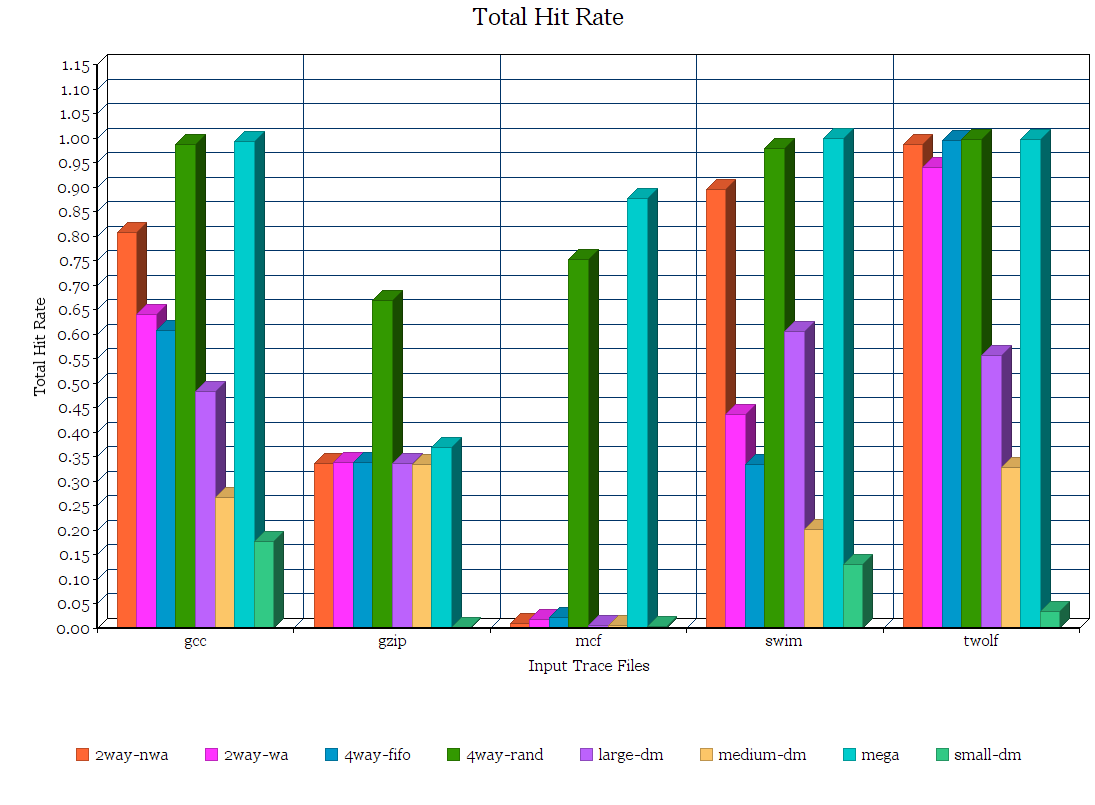
\includegraphics[scale=0.5]{hitrate}
\end{center}
\bigskip
%\pagebreak
{\bf Total Hit Rate}\\\\
Above is a graph of Total Hit Rate for all of the trace files,
run with each configuration file.
From the graph we see that 4-way-rand probably has the best trace
performance, as it's average total hit rate is 0.876,
which translates to 87.6\%. The trace file that rendered the worst
total hit rate was most likely small-dm. Analyzing its total
hit rate, we find it to have an average of 0.070, or 7.0\% total
hit rate. The other traces performed between these two extremes.
The configuration which appears to represent the average of all the
others is large-dm. Therefore if one were to be picking a
configuration based on this data alone, they would most likely
choose large-dm.
\\\\
We observe the same general trend from left to right for each
respective configuration. Looking at the performance of the
trace files as a whole, gzip appears to be the most constant;
the average total hit rate
of the gzip group of configurations is 34.0\%. The worst performance
of the trace files appears to be mcf,
which has an average of 21.2\%.
twolf seems to be the best overall trace performance. The average
value of twolf is 48.0\%, which is indeed better than gzip and mcf.
\\\\
Now we analyze the Average Memory Access Latency graph.\\
\begin{center}
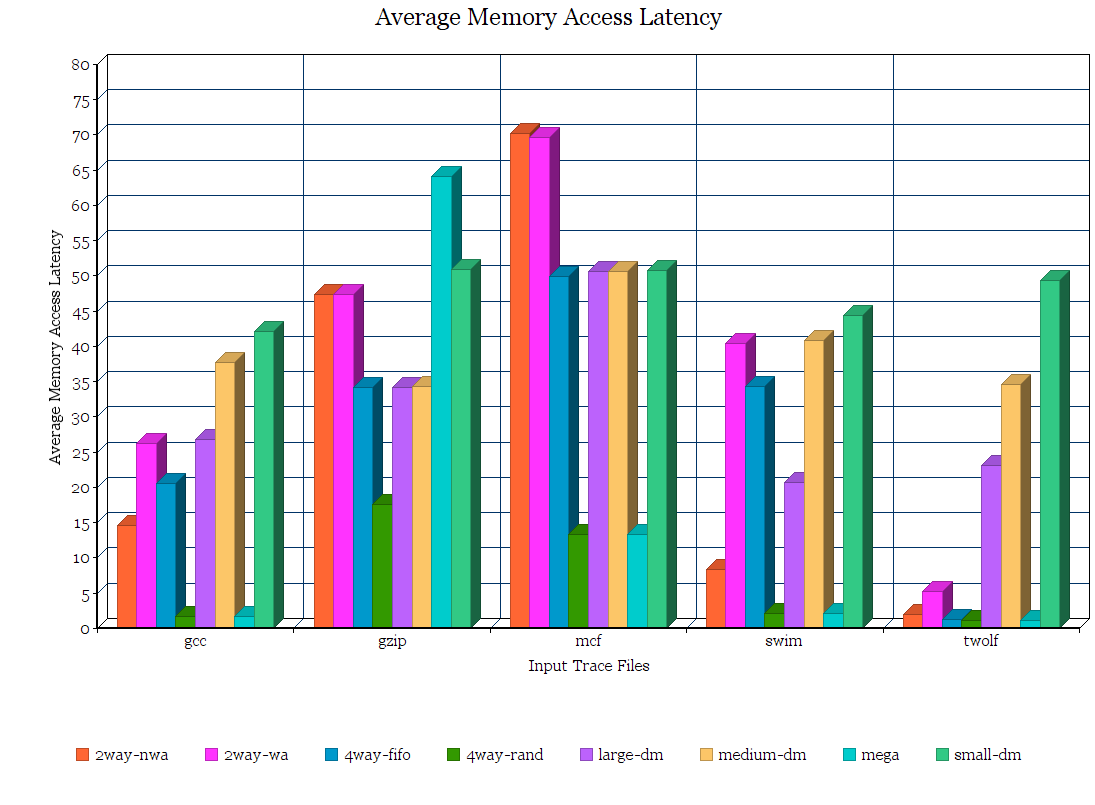
\includegraphics[scale=0.5]{latency}
\end{center}
{\bf Memory Access Latency}\\\\
Above is a graph of Average Memory Access Latency for all of the
trace files, run with each configuration file.
From the graph, it appears that small-dm has the worst average
memory access latency, with a calculated average of 30.6. This
is much worse than our data for 4way-rand, which has an average
of 4.54. The other trace files seem to fluctuate up and down,
except medium-dm appears to have the most constant performance
in all circumstances. This does not follow the trend of the others
however, as again it seems like large-dm is the most average
case of all the other configurations. If one were wanting to choose
the most efficient configuration in respect to memory latency,
they would most likely choose large-dm.
\\\\
Looking at trends in traces, we find that mcf again has the worst
overall performance. The overall average memory latency for mcf
is 46.1, which is much higher compared with twolf, with an
overall average memory latency of 14.7. The general slop of this
graph appears to follow a bell-curve, which is most likely a
coincidence from the orginization of data. However we do see
a general shape for the individual configurations
inside each trace.
\\\\
{\bf Conclusion}\\\\
Looking at our results for both the Total Hit Rate and Average
Memory Access Time, it appears that the best performing
configuration for all categories would be large-dm, and the best
performing trace would be twolf. Analyzing the worst performing
configuration, we see that this would most likely be small-dm,
and the worst performing trace is would be mcf.
%==========================================================
\end{document}
%==========================================================
